\begin{figure}[htbp]
  \centering
  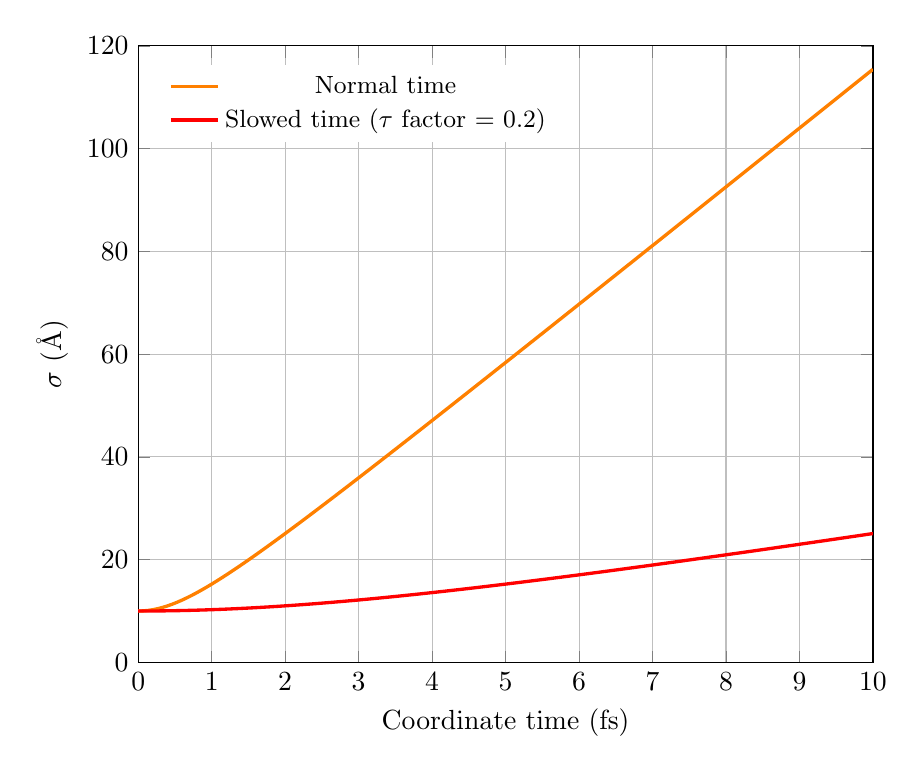
\begin{tikzpicture}
  \begin{axis}[
      width=0.9\textwidth,
      xlabel={Coordinate time (fs)},
      ylabel={$\sigma$ (\AA)},
      xmin=0, xmax=10,
      ymin=0, ymax=120,
      grid=both,
      legend style={draw=none, font=\small},
      legend pos=north west]
    % parameters
    \pgfmathsetmacro{\sigmaZero}{10}      % 0.1 nm = 10 Å
    \pgfmathsetmacro{\hbarOvermSigma}{115}% chosen so that σ=115 Å at 10 fs
    % Normal time  ---------------------------------------------
    \addplot[very thick,orange,domain=0:10,samples=150]
      {sqrt(\sigmaZero^2 + (\hbarOvermSigma*x/10)^2)};
    \addlegendentry{Normal time}
    % Slowed time  (τ factor = 0.2) -----------------------------
    \addplot[very thick,red,domain=0:10,samples=150]
      {sqrt(\sigmaZero^2 + (\hbarOvermSigma*0.2*x/10)^2)};
    \addlegendentry{Slowed time ($\tau$ factor = 0.2)}
  \end{axis}
  \end{tikzpicture}
  %-------------------------------------------------------------
  \caption{Wave-packet broadening: in a slowed-time region
           (clock rate $\times 0.2$) dispersion is five-times slower than
           under normal time.}
  \label{fig:WavePacket}
\end{figure}